\documentclass{ximera}

\title{Exercise banks}
\author{Bart Snapp}

\begin{document}
\begin{abstract}
  Ximera can present exercise banks.
\end{abstract}
\maketitle


% \section{Exercise banks}

Exercise banks can be made with \verb!xourse! files. If you are making an
exercise bank, you might want to have essentially one exercise per file.

\paragraph{File structure}

\begin{center}
  \scalebox{.7}{
    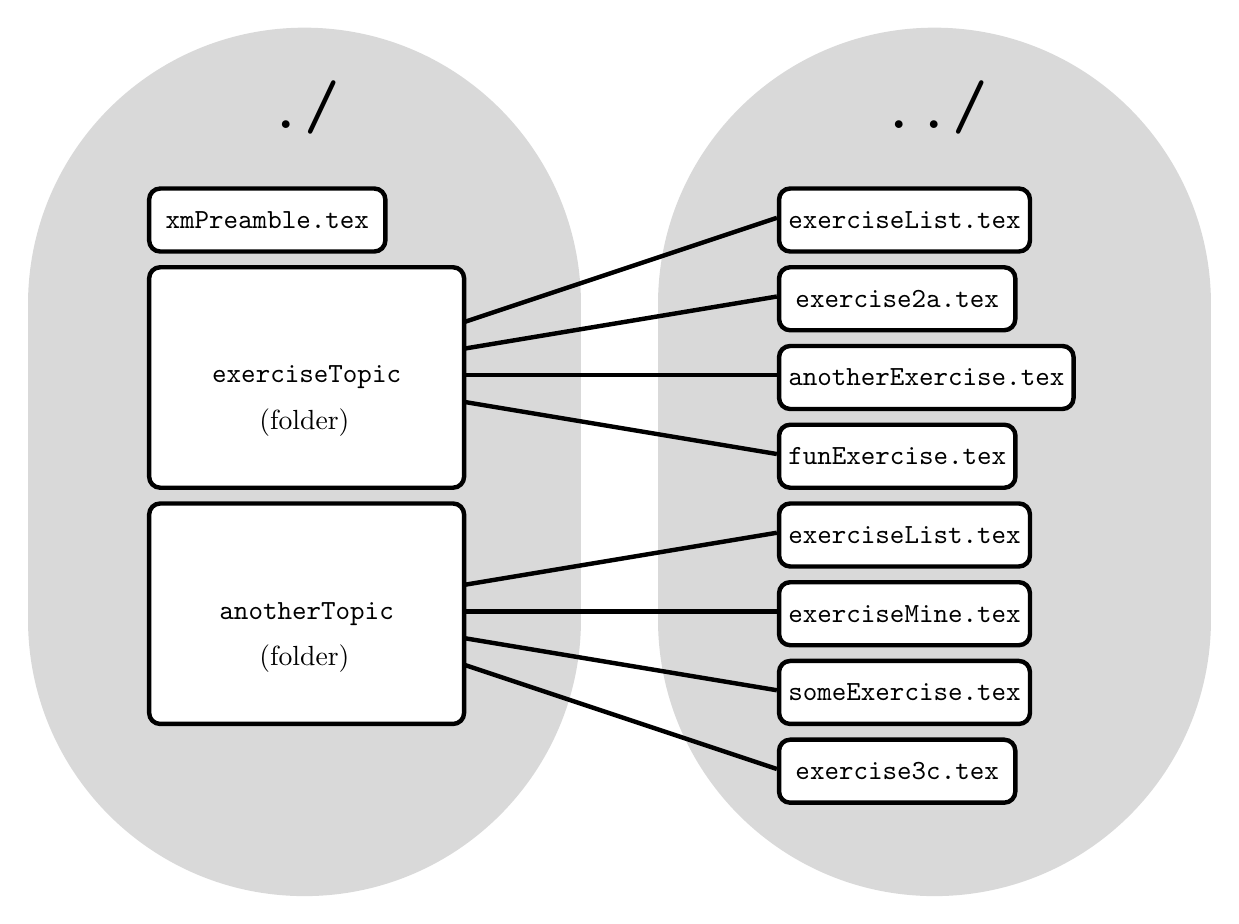
\begin{tikzpicture}
      % Define styles for nodes
      \tikzstyle{document} = [anchor=north west,draw, rounded corners,
      rectangle,
      minimum width=3cm,fill=white, minimum height=.8cm, ultra
      thick,font=\ttfamily]
      \tikzstyle{folder} = [anchor=north west,draw, rectangle, rounded corners,
      minimum width=4cm,fill=white, minimum height=2.8cm, ultra
      thick,font=\ttfamily]

      % Thick grey lines
      \draw[line width=200pt,white!85!black,line cap=round] (2,1.5) -- (2,-2.5);
      \draw[line width=200pt,white!85!black,line cap=round] (10,1.5) --
      (10,-2.5);

      % Connections
      \draw[ultra thick] (2,.6) -- (8,2.6);
      \draw[ultra thick] (2,.6) -- (8,1.6);
      \draw[ultra thick] (2,.6) -- (8,.6);
      \draw[ultra thick] (2,.6) -- (8,-.4);

      \draw[ultra thick] (2,-2.4) -- (8,-1.4);
      \draw[ultra thick] (2,-2.4) -- (8,-2.4);
      \draw[ultra thick] (2,-2.4) -- (8,-3.4);
      \draw[ultra thick] (2,-2.4) -- (8,-4.4);

      % Symbols at top
      \node at (2,4) {\Huge \tt ./};
      \node at (10,4) {\Huge \tt ../};

      % Define the folders at top level
      \node[document] at (0,3) {xmPreamble.tex};
      \node[folder] at (0,2) {exerciseTopic};
      \node[] at (2,0) {(folder)};
      \node[folder] at (0,-1) {anotherTopic};
      \node[] at (2,-3) {(folder)};

      % Define the documents in the exercises folder
      \node[document] at (8,3) {exerciseList.tex};
      \node[document] at (8,2) {exercise2a.tex};
      \node[document] at (8,1) {anotherExercise.tex};
      \node[document] at (8,0) {funExercise.tex};

      \node[document] at (8,-1) {exerciseList.tex};
      \node[document] at (8,-2) {exerciseMine.tex};
      \node[document] at (8,-3) {someExercise.tex};
      \node[document] at (8,-4) {exercise3c.tex};
    \end{tikzpicture}
  }
\end{center}

The individual exercises that live in folders might look something like:

\begin{verbatim}
\documentclass{ximera}
\author{Sophie Germain}
\begin{document}
\begin{exercise}
Compute:
\[
  \frac{\partial}{\partial x} \sin(3xyx) 
  = \answer{3yz\cos(3xyz)}
\]
\end{exercise}
\end{document}
\end{verbatim}

In this case, the \verb!exerciseList! within \verb!exerciseTopic! might look
like

\begin{verbatim}
\documentclass{xourse}
\author{Emmy Noether}
\title{My exercise banks}
\begin{document}
\begin{abstract}
Here is an exercise bank
\end{abstract}
\maketitle

\practice{exercise2a}
\practice{anotherExercise}
\practice{funExercise}

\end{document}
\end{verbatim}
If you don't give your \verb!xourse! file a title, it will not show up on the
front page.
Instead you can link directly to the file by going to something like:
\begin{center}
  \verb!https://some.ximera.server/DEPOLOY-NAME/exerciseTopic/exerciseList!
\end{center}



\end{document}
